% Eksperimentala evaluacija i rezultati

Да би се верификовале теоријске анализе временске сложености и испитала практична ефикасност предложених динамичких алгоритама над DHB структуром, спроведена је експерименатална евалуација. Евалуација је усмерена на мерење времена извршавања основних операција ажурирања графа, као и специфичних упита који се извршавају над структуром података.

\section{Експериментално окружење}

Сва мерења извршена су у контролисаном хардверском и софтверском окружењу, са циљем да се обезбеде услови за репродуктивност експеримената и смањи утицај системских фактора на измерене резултате.

\subsection{Хардверско окружење:}

\begin{itemize}

\item \emph{Процесор:} Intel Core i5-1135G7 (11th Gen, Tiger Lake) са 4 физичка језгра и 8 логичких нити, базног такта $2.40\text{ GHz}$ и максималног \textit{Boost} такта до $4.20\text{ GHz}$.
\item \emph{Кеш меморија:} L1: $320\text{ KiB}$, L2: $5\text{ MiB}$, L3: $8\text{ MiB}$.
\item \emph{Оперативна меморија:} $16\text{ GB}$ DDR4.
\item \emph{Диск:} NVMe SSD Western Digital PC SN730 $512\text{ GB}$.

\end{itemize}

\subsection{Софтверско окружење и алати:}

\begin{itemize}

\item \emph{Оперативни систем:} Linux Mint 21.3 Virginia (64-bit).
\item \emph{Преводилац:} GCC 11.4.0.
\item \emph{Систем за изградњу:} CMake 3.16+ уз стандард C++17.
\item \emph{Оптимизација:} Сви извршни фајлови коришћени у евалуацији компајлирани су у \texttt{Release} режиму, уз оптимизацију кода помоћу заставице \texttt{-O3} и искључивање \texttt{assert} провера помоћу макроа \texttt{-DNDEBUG}. Ове опције су део глобалне CMake конфигурације пројекта.

\end{itemize}

\section{Начин мерења}

За потребе емпиријске евалуације перформанси имплементираних алгоритама, пројектовано је бенчмарк окружење у језику \texttt{C++} које помоћу \texttt{std::chrono} библиотеке мери време извршавања операција додавања грана и упита над тренутним стањем графа. Улазни подаци се псеудослучајно генеришу помоћу генератора са детерминистичким почетним стањем израчунатим на основу броја чворова и итерације ради обезбеђивања репродуктивности. 

Чворови се додају у граф у серијама од по $100$ чворова, а након сваке серије се врши псеудослучајно додавање грана између чворова. Мери се укупно време додвања свих грана у серији, након чега се израчунава просечно време по грани. Након тога извршава се $10.000$ упита зависно од одабраног алгоритма, а време извршавања се такође мери и израчунава просечно време по упиту. Овај процес понавља се 5 пута са различитим почетним стањем генератора, а коначан резултат се добија као просек свих појединачних мерења. Сви резултати се бележе у CSV фајл за накнадну анализу и визуализацију.

\section{Резултати}

На слици~\ref{fig:connectivity_plot} приказани су резултати перформанси инкременталног алгоритма за динамичку повезаност. Крива просечног времена додавања гране (\texttt{avg\_add\_edge\_ns}) показује благо логаритамско увећање са порастом броја чворова $|V|$, што је у потпуности сагласносно са теоријском сложеношћу $O(\log |V|)$ оствареном применом структуре дисјунктних подскупова. Са друге стране, крива за упит повезаности (\texttt{avg\_is\_connected\_ns}) је приближно константна током целог тестног опсега, чиме се практично потврђује амортизована сложеност $O(1)$ приликом испитивања припадности чворова истој компоненти повезаности.

\begin{figure}[h]
\centering
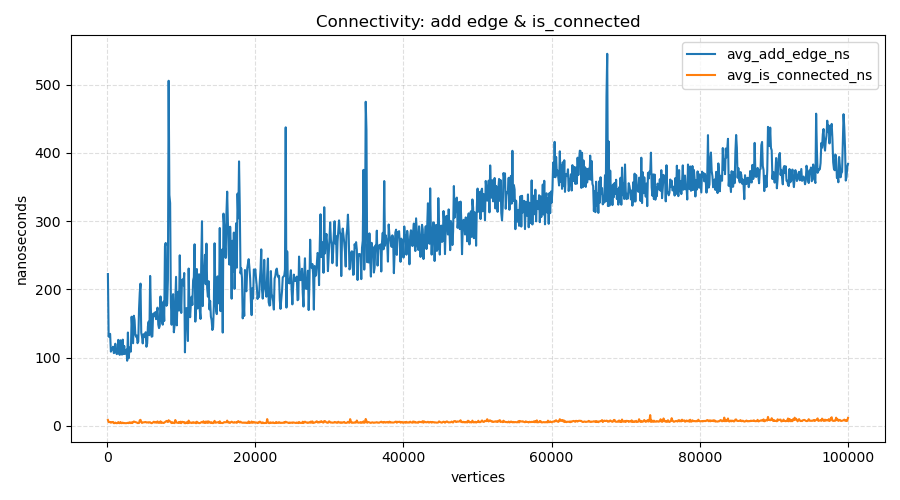
\includegraphics[width=1\textwidth]{images/connectivity_plot.png}
\caption{Резултати мерења за динамичку повезаност}
\label{fig:connectivity_plot}
\end{figure}

Резултати експерименталне евалуације за алгоритам одржавања динамичког минималног разапињућег стабла приказани су на слици~\ref{fig:mst_plot}. Време извршавања операције додавања гране која у себи укључује и реконструкције разапињуће шуме (\texttt{avg\_add\_edge\_ns}) показује приблично линеарни тренд раста у односу на број чворова $|V|$, што верно рефлектује изведену сложеност $O((|V|+|E|) \log |V|)$. Операција провере припадности гране минималном разапињућем стаблу (\texttt{avg\_is\_in\_mst\_ns}) показује стабилне и занемарљиве временске варијације, што потврђује ефикасност директног претраживања заснованог на хеш-индексирању у времену $O(1)$. 

\begin{figure}[h]
\centering
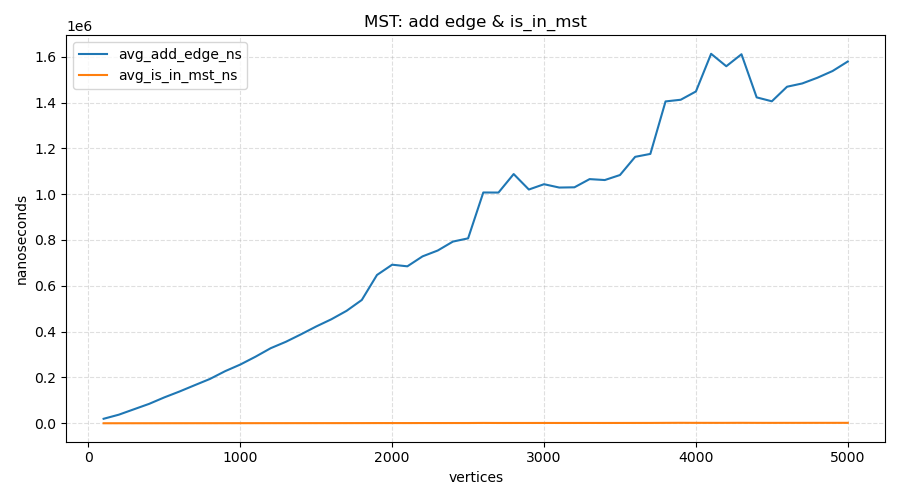
\includegraphics[width=1\textwidth]{images/mst_plot.png}
\caption{Резултати мерења за динамичко минимално разапињуће стабло}
\label{fig:mst_plot}
\end{figure}

На слици~\ref{fig:suitor_plot} приказано је временско понашање Суитор алгоритма. Мерења показују да време додавања гране (\texttt{avg\_add\_edge\_ns}) показује приближно линеарну зависност у односу на број чворова, што директно одговара теоријској сложености $O(|V|)$. Упит за проверу статуса упарености произвољног чвора (\texttt{avg\_is\_matched\_ns}) остаје на занемарљивој вредности током свих тестова, чиме се потврђује константна сложеност.

\begin{figure}[h]
\centering
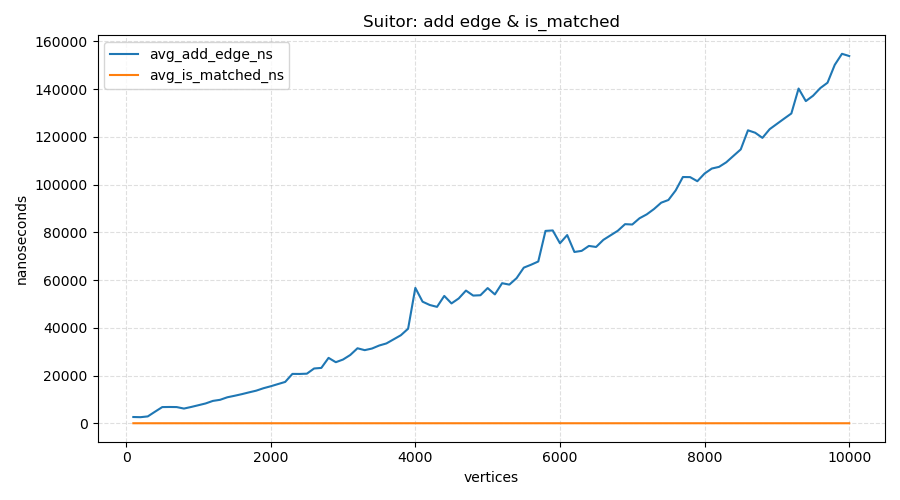
\includegraphics[width=1\textwidth]{images/suitor_plot.png}
\caption{Резултати мерења за Суитор алгоритам}
\label{fig:suitor_plot}
\end{figure}

% Eksperimentala evaluacija i rezultati